\begin{example}
    Пусть $p_n$ – простое $n$-ое число. Рассмотрим $\prod \limits_{k=1}^\infty \frac{p_k}{p_k-1}=\prod \limits_{k=1}^\infty \frac{1}{1-\frac{1}{p_k}}$ – расходится. Более того, $\prod \limits_{k=1}^n \frac{p_k}{p_k-1}\geq H_n$ – $n$-ое гармоническое число.

    $\prod \limits_{k=1}^n \frac{1}{1-\frac{1}{p_k}}> \prod \limits_{k=1}^n\sum\limits_{j=1}^n\frac{1}{p_k^j}=\sum \frac{1}{p_1^{\alpha_1}\cdot p_n^{\alpha_n}}\geq \sum\limits_{m=1}^n\frac{1}{m}=H_n\rightarrow +\infty$
    
    $0\leq \alpha_1, ..., \alpha_n\leq n$

    $\frac{1}{1-x}> \sum\limits_{k=1}^n x_k$ при $0<x<1$.
\end{example}

\begin{theorem}
    Ряд $\sum\limits_{n=1}^{+\infty}\frac{1}{p_n}$ расходится. Более того $\sum\limits_{k=1}^{n}\frac{1}{p_k}\geq \ln \ln n - 1$.
\end{theorem}

\begin{proof}
    $\prod\limits_{k=1}^n\frac{1}{1-\frac{1}{p_k}}=\prod\limits_{k=1}^n\frac{p_k}{p_k-1}\geq H_n$

    $\sum\limits_{k=1}^n-\ln(1-\frac{1}{p_k})\geq \ln H_n$

    Докажем: $-\ln(1-\frac{1}{p_k})\leq \frac{1}{p_k}+\frac{1}{p_k^2}$

    $-\ln(1-t)\leq t+t^2$ при $0\leq t \leq \frac{1}{2}$

    $\frac{1}{1-t}\leq 1+2t\quad (1\leq (1+2t)(1-t)=1+t-2t^2$)

    Тогда: $\sum \limits_{k=1}^n\frac{1}{p_k} + \sum \limits_{k=1}^n \frac{1}{p_k^2} \geq \sum \limits_{k=1}^n-\ln(1-\frac{1}{p_k})\geq \ln H_n\geq \ln\ln n$

    Поймем, что слева за константа: $\sum \limits_{k=1}^n \frac{1}{p_k^2}\leq \sum \limits_{k=1}^n\frac{1}{k^2}\leq \sum \limits_{k=1}^n\frac{1}{k(k-1)} = 1 - \frac{1}{n}$
\end{proof}

\begin{remark}
    На самом деле $\sum \limits_{k=1}^n \frac{1}{p_k}=\ln\ln n + \mathcal{O}(1)$.
\end{remark}

\begin{exercise}~
    \begin{enumerate}
        \item $\sum\limits_{k\leq p\leq k^2, p\text{ – простое}}\leq \frac{4}{3}$
        \item $\sum\limits_{p\leq n}\leq 2 \ln \ln n + 4$
    \end{enumerate}
\end{exercise}

\subsection{Функциональные последовательности и ряды}

\begin{definition}
    Пусть $f, f_n:E\rightarrow \R$. $f_n$ \textit{сходятся к $f$ поточечно}, если $\lim f_n(x)=f(x)\  \forall x\in E$.
\end{definition}

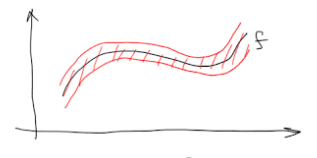
\includegraphics[width=0.4\linewidth]{images/19-04-1.png}

\begin{definition}
    Пусть $f, f_n : E \rightarrow \R$. $f_n$ \textit{сходятся к $f$ равномерно на $E$} ($f_n\rightrightarrows f$), если $\forall \varepsilon > 0\ \exists \underset{=N(\varepsilon)}{N}: \forall n\geq N\ \forall x\in E\ |f_n(x)-f(x)|< \varepsilon$.
\end{definition}

\begin{remark}
    Поточечная сходимость с помощью $\varepsilon-N$: $\forall x\in E\ \forall \varepsilon > 0\ \exists \underset{=N(\varepsilon, x)}{N}: \forall n\geq N\ |f_n(x)-f(x)|< \varepsilon$.
\end{remark}

\begin{remark}
    $f_n(x)=x^n\quad E=(0, 1)\quad f(x)\equiv 0$

    $\lim f_n(x)=f(x)\quad \forall x\in (0, 1)$ – поточечная сходимость есть.

    Заметим, что если есть равномерная сходимость, то поточечная тоже есть к такой же функции (нашлась такая универсальная, которая точно подойдет под условия поточечной сходимости). Пусть $f_n\rightrightarrows 0$. Тогда $ \forall \varepsilon > 0\ \exists N\ \forall n \geq N\ \underbrace{\forall x\in (0, 1)\ x^n< \varepsilon}_{\text{так не бывает}}\Rightarrow$  равномерной сходимости нет.
\end{remark}

\begin{theorem}
    Пусть $f, f_n:E\rightarrow \R$. Тогда $f_n \rightrightarrows f$ на $E\Leftrightarrow \sup\limits_{x\in E}|f_n(x)- f(x)|\underset{n\rightarrow \infty}{\rightarrow} 0$.
\end{theorem}

\begin{proof}~
    \begin{enumerate}
        \item[$\Rightarrow$] $f_n \rightrightarrows f\Rightarrow \forall \varepsilon > 0\ \exists \underset{=N(\varepsilon)}{N}: \forall n\geq N\ \underbrace{\forall x\in E\ |f_n(x)-f(x)|< \varepsilon}_{\Rightarrow \sup\limits_{x\in E}|f_n(x)-f(x)|\leq \varepsilon}$

        $\forall \varepsilon > 0\ \exists \underset{=N(\varepsilon)}{N}: \forall n\geq N\ \sup\limits_{x\in E}|f_n(x)-f(x)|\leq \varepsilon \Rightarrow \sup\limits_{x\in E}|f_n(x_-f(x)|\rightarrow 0$
        \item[$\Leftarrow$] $\sup\limits_{x\in E}|f_n(x)-f(x)|\rightarrow 0 \Rightarrow \forall \varepsilon > 0\ \exists \underset{=N(\varepsilon)}{N}: \forall n\geq N\ \sup\limits_{x\in E}\underset{\geq |f_n(x)-f(x)|\quad \forall x\in E}{|f_n(x)-f(x)|}< \varepsilon \Rightarrow \forall \varepsilon > 0\ \exists \underset{=N(\varepsilon)}{N}: \forall n\geq N\ \forall x\in E\ |f_n(x)-f(x)|< \varepsilon\Rightarrow f_n \rightrightarrows f$
    \end{enumerate}
\end{proof}

\begin{corollary}~
    \begin{enumerate}
        \item Если $|f_n(x)-f(x)|\leq a_n\ \forall x\in E$ и $\lim a_n=0\Rightarrow f_n \rightrightarrows f$  на $E$.
        \begin{proof}
            $\sup\limits_{x\in E}|f_n(x)-f(x)|\leq a_n\rightarrow 0$
        \end{proof}
        \item Если существуют $x_n\in E: \underbrace{f_n(x_n)-f(x_n)}_{=:b_n}\not \rightarrow 0$, то нет равномерной сходимости.
        \begin{proof}
            $\sup\limits_{x\in E}|f_n(x)-f(x)|\geq |b_n|$ (значение в какой-то точке)
            
            $|b_n|\not\rightarrow 0\Rightarrow$ $\exists b_{n_k}: |b_{n_k}|>\delta>0 \Rightarrow \sup ... > \delta$ и $\not\rightarrow 0$.
        \end{proof}
    \end{enumerate}
\end{corollary}

\begin{definition}
    Пусть $f_n: E\rightarrow \R$. Последовательность $f_n$ \textit{равномерно ограничена}, если $\exists M$, т.ч. $\forall n\ \forall x\in E\ |f_n(x)|\leq M.$
\end{definition}

\begin{theorem}
    Пусть $f_n$ равномерно ограничена, $g_n\rightrightarrows 0\Rightarrow f_ng_n\rightrightarrows 0$ .
\end{theorem}

\begin{proof}
    Если $|f_n(x)g_n(x)|\leq M|g_n(x)|$, то и $\sup\limits_{x\in E}|f_n(x)g_n(x)|\leq \sup\limits_{x\in E}|g_n(x)|\cdot M\rightarrow 0$.
\end{proof}

\begin{theorem}
    \textbf{Критерий Коши для равномерной сходимости последовательности функций.}

    Пусть $f_n:E\rightarrow \R$. Тогда $f_n$ равномерно сходится на $E$ у некоторой функции $\Leftrightarrow \forall \varepsilon > 0\ \exists N\ \forall n, m\geq N\ \forall x\in E\ |f_n(x)-f_m(x)|<\varepsilon$.
\end{theorem}

\begin{proof}~
    \begin{enumerate}
        \item[$\Rightarrow$.] Пусть $f_n\rightrightarrows f$ на $E$.

        $\left.\begin{array}{l}
           \forall \varepsilon > 0\ \exists N\ \forall n\geq N\ \forall x\in E\ |f_n(x)-f(x)|<\frac{\varepsilon}{2}    \\
             \forall \varepsilon > 0\ \exists N\ \forall m\geq N\ \forall x\in E\ |f_m(x)-f(x)|<\frac{\varepsilon}{2}
        \end{array}\right\}\Rightarrow$

        $\Rightarrow |f_n(x)-f_m(x)|\leq |f_n(x)-f(x)|+ |f_m(x)-f(x)|<\frac{\varepsilon}{2} + \frac{\varepsilon}{2} = \varepsilon\quad x\in E$.

        \item[$\Leftarrow$.] Зафиксируем $x\in E$.

        $\forall \varepsilon > 0\ \exists N\ \forall n, m\geq N\ \forall x\in E\ |f_n(x)-f_m(x)|<\varepsilon\Rightarrow f_n(x)$ – фундаментальная последовательность вещественных чисел (для каждого конкретного аргумента) $\Rightarrow$ она имеет конечный предел $f(x):=\lim f_n(x)$.

        $\forall \varepsilon > 0\ \exists N\ \forall n, m\geq N\ \forall x\in E\ \underset{\underset{m\rightarrow \infty}{\rightarrow}|f_n(x)-f(x)|\leq \varepsilon}{|f_n(x)-f_m(x)|}<\varepsilon\Rightarrow f_n \rightrightarrows f$ на $E$.
    \end{enumerate}
\end{proof}

\begin{definition}
    \textit{Пространство} $l^\infty (E):=\{f\mid f:E\rightarrow \R\text{  – ограниченная}\}$.

    $\|f\|_{l^\infty (E)}=\|f\|_\infty:= \sup\limits_{x\in E} |f(x)|$ – \textit{норма}.
\end{definition}

\begin{remark}
    Несложно проверить, что это норма: неотрицательность, $\sup = 0 \Rightarrow f\equiv 0$, выносимость константы – очевидно.

    Неравенство треугольника тоже банально.
\end{remark}

\begin{definition}
    Пространство $C(K):=\{f \mid f:K\rightarrow \R\text{ – непрерывная}\}$.

    $\|f\|_{C(K)}=\|f\|_\infty: \max\limits_{x\in K} |f(x)|$
\end{definition}

\begin{remark}
    $C(K)\subset l^\infty (K)$ – непрерывная функция на компакте ограничена и нормы совпадают ($\sup$ и $\max$ – это одно и то же).
\end{remark}

\begin{theorem}
    $l^\infty (E)$ – полное пространство.
\end{theorem}

\begin{proof}
    Пусть $f_n\in l^\infty (E)$ – фундаментальная последовательность.

    $\forall \varepsilon > 0\ \exists N\ \forall n, m\geq N\ \forall x\in E\ \|f_n(x)-f_m(x)\|<\varepsilon$

    $\|f_n(x)-f_m(x)\|=\sup\limits_{x\in E}|f_n(x)-f_m(x)|\geq |f_n(x)-f_m(x)|\quad \forall x\in E$

    $\Rightarrow \forall \varepsilon > 0\ \exists N\ \forall n, m\geq N\ \forall x\in E\ |f_n(x)-f_m(x)|<\varepsilon\overset{\text{крит. Коши}}{\Rightarrow}$ найдется $f:E\rightarrow \R$, т.ч. $ f_n\rightrightarrows f$ на $E$, то есть $\sup\limits_{x\in E}\underset{=\|f_n-f\|}{|f_n(x)-f_m(x)|}\rightarrow 0$ (то есть сходимость по норме).

    Осталось понять, что $f\in l^\infty(E)$, то есть ограниченная функция. 

    Возьмем $n$, для которого $|f_n(x)-f(x)|<1\quad \forall x\in E\Rightarrow |f(x)|< 1 + |f_n(x)|\leq C$ так как $f_n$ – ограниченная функция.
\end{proof}

\begin{theorem}
    Пусть $f_n, f:E\rightarrow \R$, $f_n$ непрерывна в точке $a$ и $f_n\rightrightarrows f$ на $E$. Тогда $f$ непрерывна в точке $a$. 
\end{theorem}

\begin{proof}
    Возьмем $\varepsilon>0$ и будем искать для него $\delta>0$ из окрестности непрерывности $f$.

    $|f(x)-f(a)|\leq \underbrace{|f(x)-f_n(x)|}_{<\varepsilon}+\underbrace{|f_n(x)-f_n(a)|}_{<\varepsilon}+\underbrace{|f_n(a)-f(a)|}_{<\varepsilon}<3\varepsilon$

    $\exists N\ \forall n\geq N\ \forall x\in E\ |f_n(x)-f(x)|<\varepsilon$. 
    
    Возьмем любое $n\geq N$. Тогда $|f_n(x)-f(x)|<\varepsilon$ и $|f_n(a)-f(a)|<\varepsilon$.

    Знаем, что $f_n$ непрерывна в точке $a\Rightarrow \exists \delta>0 : \forall |x-a|<\delta\Rightarrow |f_n(x)-f_n(a)|<\varepsilon$.

    Нашли подходящую $\delta >0$.
\end{proof}

\begin{corollary}
    \textbf{Теорема Стокса-Зайделя.}

    Пусть $f_n\in C(E)$ и $f_n\rightrightarrows f$ на $E$. Тогда $f\in C(E)$.

    (Предыдущая теорема, примененная во всех точках по отдельности)
\end{corollary}

\begin{corollary}
    $C(K)$ – замкнутое подпространство $l^\infty(K)$.
\end{corollary}

\begin{proof}
    $\|f_n - f\|_\infty\rightarrow 0\Leftrightarrow\sup\limits_{x\in E}|f_n(x)-f(x)|\rightarrow 0\text{ (расшифровка нормы) }\Leftrightarrow f_n\rightrightarrows f$ на $E$.

    По предыдущей теореме равномерная сходимость непрерывность не портит $\Rightarrow$ мы не вылезем за пределы непрерывных функций.
\end{proof}

\begin{theorem}
    Пусть $(X, \rho)$ – полное метрическое пространство, $Y\subset X$ – замкнутое. Тогда $(Y, \rho)$ – полное.
\end{theorem}

\begin{proof}
    Возьмем фундаментальную последовательность $y_n\in Y\Rightarrow$ она фундаментальная в $(X, \rho)\text{  (метрика та же самая) }\overset{X \text{ – полное}}{\Rightarrow}$ найдется $x\in X$, т.ч. $ \lim y_n=x\Rightarrow x$ – предельная точка $Y\Rightarrow x\in Y$, так как $Y$ – замкнуто.
\end{proof}

\begin{corollary}
    $C(K)$ –  полное.
\end{corollary}

\begin{remark}
    Поточечная сходимость не сохраняет непрерывность.
\end{remark}

\begin{example}
    Рассмотрим $f_n(x)=x^n$ на $(0, 1]$.
    
    Она поточечно сходится к $f(x) =\left\{\begin{array}{ll} 0,&\text{ при } x\in (0, 1) \\ 1,&\text{ при } x=1
    \end{array}\right.$ – непрерывность испортилась.
\end{example}

\begin{definition}
    Пусть $u_k:E\rightarrow \R$. Ряд $\sum\limits_{k=1}^\infty u_k$ \textit{сходится поточечно}, если $\forall x\in E$ ряд $\sum\limits_{k=1}^\infty u_k(x)$ сходится $\Leftrightarrow S_n(x)=\sum\limits_{k=1}^n u_k(x)$ поточечно сходится.
\end{definition}

\begin{definition}
    Ряд \textit{сходится равномерно} на $E$, если $S_n(x)$ сходятся равномерно на $E$.
\end{definition}

\begin{definition}
    Пусть $\sum\limits_{k=1}^\infty u_k(x)$ сходится поточечно, $u_k:E\rightarrow \R$. \textit{Остаток ряда} $r_n(x):=\sum\limits_{k=n+1}^\infty u_k(x): E\rightarrow \R$.
\end{definition}

\begin{remark}
    $S_n(x)+r_n(x)=\sum\limits_{k=1}^\infty u_k(x)=:S(x)$ – сумма ряда.
\end{remark}

\begin{theorem}
    \textbf{Необходимое условие равномерной сходимости ряда.}

    Пусть $\sum\limits_{k=1}^\infty u_k(x)$ сходится поточечно. Тогда $\sum\limits_{k=1}^\infty u_k(x)$ сходится равномерно $\Leftrightarrow r_n\rightrightarrows 0$.
\end{theorem}

\begin{proof}
    $S(x)-S_n(x)=r_n(x)\rightrightarrows 0\Leftrightarrow S_n \rightrightarrows S$
\end{proof}

\begin{remark}~
    \begin{enumerate}
        \item Если ряд сходится равномерно, то $u_n\rightrightarrows 0$ (полный аналог необходимого условия сходимости числового ряда, только здесь равномерная сходимость и равномерное стремление к нулю).
        \begin{proof}
            $S_n\rightrightarrows S\Rightarrow u_n=S_n-S_{n-1}\rightrightarrows S - S = 0$
        \end{proof}
        \item Если найдутся $x_n\in E: \underbrace{u_n(x_n)\not \rightarrow 0}_{\Rightarrow\text{ нет }\rightrightarrows 0}$, то нет равномерной сходимости ряда $\sum\limits_{k=1}^\infty u_k(x)$. 
        \item Если найдутся $x_n\in E: \sum\limits_{k=1}^\infty u_k(x)$ расходится, то это вообще ничего не значит.
        \begin{example}
            $u_n(x)=\left\{\begin{array}{ll} \frac{1}{n},&\text{ при } x\in [\frac{1}{n+1}, \frac{1}{n}) \\ 0,&\text{  иначе}
    \end{array}\right.$

        $x_n=\frac{1}{n+1}$, $u_n(x_n)=\frac{1}{n}$, $\sum u_n(x_n)=\sum \frac{1}{n}$ – расходится.

        $\sum\limits_{n=1}^\infty u_n(x)$ равномерно сходится, $0\leq r_n(x)\leq \frac{1}{n}$
        \end{example}
    \end{enumerate}
\end{remark}

\begin{theorem}
    \textbf{Критерий Коши для равномерной сходимости функционального ряда.}

    Пусть $u_k: E\rightarrow \R$. Тогда $\sum\limits_{k=1}^\infty u_k$ сходится равномерно на $E\Leftrightarrow \forall \varepsilon > 0\ \exists N\ \forall n> m\geq N\ \forall x\in E\ |\sum\limits_{k=m+1}^n u_k|< \varepsilon$.
\end{theorem}

\begin{proof}
    $\sum\limits_{k=1}^\infty u_k$ сходится равномерно на $E\Leftrightarrow S_n\rightrightarrows S $ на $E\overset{\text{крит. Коши}}{\Leftrightarrow} \forall \varepsilon > 0\ \exists N\ \forall n> m\geq N\ \forall x\in E\ |\underbrace{S_n(x)-S_m(x)}_{=\sum\limits_{k=m+1}^n u_k}|<\varepsilon$
\end{proof}

\begin{theorem}
    \textbf{Признак сравнения.}

    Пусть $|u_n(x)|\leq v_n(x)\ \forall x\in E\ \forall n$. Тогда если $\sum\limits_{n=1}^\infty v_n(x)$ сходится равномерно, то и $\sum\limits_{n=1}^\infty u_n(x)$ сходится равномерно.
\end{theorem}
\begin{proof}
    $\sum\limits_{n=1}^\infty v_n(x)$ сходится равномерно $\overset{\text{крит. Коши}}{\Rightarrow} \forall \varepsilon > 0\ \exists N\ \forall n> m\geq N\ \forall x\in E\ \underbrace{|\sum\limits_{k=m+1}^n v_k(x)|}_{\geq \sum\limits_{k=m+1}^n |u_k(x)|\geq |\sum\limits_{k=m+1}^n u_k(x)|}<\varepsilon\Rightarrow\forall \varepsilon > 0\ \exists N\ \forall n> m\geq N\ \forall x\in E\ |\sum\limits_{k=m+1}^n u_k(x)|<\varepsilon\overset{\text{крит. Коши}}{\Rightarrow}$
    
    $\Rightarrow\sum\limits_{n=1}^\infty u_n(x)$ сходится равномерно.
\end{proof}

\begin{remark}
    Должно напоминать факт, что из абсолютной сходимости ряда следует обычная.
\end{remark}

\begin{corollary}
    \textbf{Признак Вейерштрасса.}

    Если $|u_n(x)|\leq a_n\ \forall x\in E\ \forall n$ и числовый ряд $\sum\limits_{n=1}^\infty a_n$ сходится, то $\sum\limits_{n=1}^\infty u_n(x)$ сходится равномерно на $E$.
\end{corollary}

\begin{proof}
    Возьмем $v_n(x)=a_n$. Тогда $v_n(x)$ сходятся равномерно, так как от $x$ не зависят.
\end{proof}

\begin{corollary}
    Если ряд $\sum\limits_{n=1}^\infty |u_n(x)|$ сходится равномерно, то $\sum\limits_{n=1}^\infty u_n(x)$ сходится равномерно.
\end{corollary}

\begin{proof}
    Возьмем $v_n(x)=|u_n(x)|$. 
\end{proof}

\begin{example}
    $\sum\limits_{n=1}^\infty \frac{\sin nx}{n^2}$ сходится равномерно на $\R$: $|\frac{\sin nx}{n^2}|\leq \frac{1}{n^2}$ и $\sum\limits_{n=1}^\infty \frac{1}{n^2}$ сходится.
\end{example}

\begin{remark}
    Абсолютная и равномерная сходимости – разные вещи. 
    \begin{enumerate}
        \item Может быть абсолютная сходимость, но не быть равномерной.
        \begin{example} $\sum\limits_{n=1}^\infty x^n$ на $(0, 1)$ \end{example}
        \item Может быть равномерная сходимость, но не быть абсолютной.
        \begin{example} $\sum\limits_{n=1}^\infty \frac{(-1)^n}{n}$ \end{example}
        \item Может быть равномерная сходимость, абсолютная сходимость, но $\sum\limits_{n=1}^\infty |u_n(x)|$ сходится равномерно.
    \end{enumerate}
\end{remark}

\begin{theorem}
    \textbf{Признак Дирихле.}

    $\left \{\begin{array}{l}
         |\sum\limits_{k=1}^\infty a_k(x)|\leq K\quad \forall x\in E\ \forall n \\
         b_n\rightrightarrows 0\text{ на }E \\
         b_n(x)\text{ монотонны по }n\text{ для любого фикс. }x
    \end{array}\right.\Rightarrow \sum\limits_{k=1}^\infty a_k(x)b_k(x)$ равномерно сходится.
\end{theorem}

\begin{proof}
    Напишем преобразование Абеля: $\sum\limits_{k=1}^n a_k(x)b_k(x)=A_n(x)b_n(x)+\sum\limits_{k=1}^{n-1}A_k(x)(b_k(x)-b_{k+1}(x))$, где $A_k(x)=\sum\limits_{j=1}^ka_j(x)$.

    Надо доказать, что частичные суммы равномерно сходятся, то есть что каждое слагаемое в правой части равномерно сходится.

    $A_n(x)b_n(x)\rightrightarrows 0$ (равномерно ограниченная на равномерно стремящуюся к 0)

    Осталось доказать, что $\sum\limits_{k=1}^{n-1}A_k(x)(b_k(x)-b_{k+1}(x))$ равномерно сходится. Проверим, что есть равномерная сходимость ряда $\sum\limits_{k=1}^{n-1}|A_k(x)||b_k(x)-b_{k+1}(x)|$.

    $|A_k(x)||b_k(x)-b_{k+1}(x)|\leq K|b_k(x)-b_{k+1}(x)|$, поэтому осталось доказать, что $\sum\limits_{k=1}^{n-1}|b_k(x)-b_{k+1}(x)|$ равномерно сходится.

    $\sum\limits_{k=1}^{n-1}|b_k(x)-b_{k+1}(x)|=|\sum\limits_{k=1}^{n-1}b_k(x)-b_{k+1}(x)|$ ($b_n$ монотонные, то есть разности одного знака) $=|b_1(x)-b_{n+1}(x)|\rightrightarrows |b_1(x)|$
\end{proof}

\begin{theorem}
    \textbf{Признак Абеля.}

    $\left\{\begin{array}{l}
        |\sum\limits_{k=1}^\infty a_k(x)|\text{ равномерно сходится на }E\\
         b_n\text{ равномерно ограничены на }E\\
         b_n(x)\text{ монотоннны по }n\text{ для любого фикс. }x\in E
    \end{array}\right.\Rightarrow \sum\limits_{k=1}^\infty a_k(x)b_k(x)$ равномерно сх-ся на $E$.
\end{theorem}

\begin{proof}
    Хотим понять, что при больших $n$ такая сумма маленькая, напишем критерий Коши: $\sum\limits_{k=n+1}^{n+p}a_k(x)b_k(x)=\sum\limits_{k=1}^pa_{n+k}(x)b_{n+k}(x)\overset{\text{пр. Абеля}}{=}(A_{n+p}(x)-A_n(x))b_{n+p}(x)+\sum\limits_{k=1}^{p-1}(A_{n+k}(x)-A_n(x))(b_{n+k}(x)-b_{n+k+1}(x))$

    $\sum\limits_{k=1}^p a_{n+k}(x)=A_{n+p}(x)-A_n(x)$

    $|\sum\limits_{k=n+1}^{n+p}a_k(x)b_k(x)|\leq \underbrace{|(A_{n+p}(x)-A_n(x)|}_{< \varepsilon\text{ если } n\geq N}\cdot \underbrace{|b_{n+p}(x)|}_{\leq M}+\sum\limits_{k=1}^{p-1}\underbrace{|A_{n+k}(x)-A_n(x)|}_{< \varepsilon\text{ если }n\geq N}\cdot |b_{n+k}(x)-b_{n+k+1}(x)|\overset{(*)}{\leq}$

    $b_n$ равномерно ограничены $\Rightarrow |b_n(x)|\leq M$.

    $A_n(x)$ равномерно сходится $\Rightarrow\exists N\ \forall m> n\leq N\ \forall x\in E\ |A_m(x)- A_n(x)|<\varepsilon $, рассмотрим только такие $n, m$:

    $\overset{(*)}{\leq} \varepsilon M +\varepsilon \sum\limits_{k=1}^{p-1} |b_{n+k}(x)-b_{n+k+1}(x)|=\varepsilon M +\varepsilon| \sum\limits_{k=1}^{p-1} b_{n+k}(x)-b_{n+k+1}(x)|\leq \varepsilon M + \varepsilon|b_{n+1}(x)-b_{n+p+1}(x)|\leq \varepsilon M + 2\varepsilon M=3\varepsilon M$
\end{proof}

\begin{theorem}
    \textbf{Признак Лейбница.}

    Пусть $b_n(x)\geq 0$ и монотонно убывают $\forall x\in E$, $b_n\rightrightarrows 0$ на $E$. Тогда $\sum\limits_{n=1}^\infty (-1)^{n-1}b_n(x)$ равномерно сходятся на $E$.
\end{theorem}

\begin{proof}
    $a_n(x)=(-1)^{n-1}$ и подставляем в Дирихле.
\end{proof}

\begin{example}
    $\sum\limits_{n=1}^\infty \frac{(-1)^{n-1}x^n}{n}$ на $(0, 1)$ сходится равномерно: 
    
    $b_n(x)=\frac{x^n}{n}\geq 0$, $0\leq b_n(x)\leq \frac{1}{n}\Rightarrow b_n\rightrightarrows 0$ и признак Лейбница.

    $\sum\limits_{n=1}^\infty |\frac{(-1)^{n-1}x^n}{n}|=\sum\limits_{n=1}^\infty\frac{x^n}{n}$ сходится неравномерно: 
    
    Применим критерий Коши: $\forall \varepsilon > 0\ \exists N\ \forall m> n\geq N\ \forall x\in (0, 1)\ \sum\limits_{k=n+1}^m \frac{x^k}{k}<\varepsilon$

    $m=2n\ x\rightarrow 1_-\quad \frac{1}{2}< \frac{x^k}{k}<\varepsilon$

    Вот тот самый пример, когда абсолютная есть, равномерная есть, но у суммы модулей равномерная исчезает.
\end{example}

\begin{theorem}
    \textbf{Признак Дини.}

    Пусть $K$ – компакт, $u_n\in C(K)$, $u_n\geq 0$ и $S(x)=\sum\limits_{k=1}^\infty u_k(x)\in C(K)$. Тогда $\sum\limits_{n=1}^\infty u_k (x)$ сходится равномерно на $K$.
\end{theorem}
\begin{proof}
    $r_n(x)=\sum\limits_{k=n+1}^\infty u_k(x)\quad r_n(x)=r_{n+1}(x)+u_{n+1}(x)\geq r_{n+1}(x)\Rightarrow r_n(x)\geq 0$ и монотонно убывают.

    Надо доказать, что $\forall \varepsilon > 0\ \exists n\ \forall x\in K \ r_n(x) < \varepsilon$.
    
    Пусть никакое $n$ не подходит, то есть $\forall n\ \exists x_n\in K$, т.ч. $r_n(x_n)\geq \varepsilon$

    $x_n$ – последовательность компакта $\Rightarrow$ найдется сходящаяся подпоследовательность $x_{n_k}$, $x_0:=\lim x_{n_k}$.

    $r_n$ непрерывно в точке $x_0$ так как $ r_n(x)=S(x)-S_n(x)$, где $S(x)$ непрерывно по условию, а $S_n(x)$ – конечное число непрерывных слагаемых.

    Тогда знаем, что $r_m(x_0)\underset{k\rightarrow\infty}{\leftarrow} r_m(x_{n_k})\underset{\text{так как } r_n\searrow}{\geq r_{n_k}(x_{n_k})}$ $\geq \varepsilon\Rightarrow r_m(x_0)\geq \varepsilon\quad \forall m$. Тогда в этой точке нет стремления к нулю. Противоречие с тем, что ряд сходится в точке $x_0$.
\end{proof}